\documentclass[letterpaper,10pt]{article}

\usepackage[utf8]{inputenc}
\usepackage[spanish]{babel}
\usepackage{fontenc}
\usepackage[dvipdfmx]{graphicx}
\usepackage{bmpsize,wrapfig,xcolor}
\usepackage{fullpage}
\usepackage{amssymb}
\usepackage[hidelinks]{hyperref}

% Para evitar que se indente solo a cada rato
\setlength\parindent{0pt}

\begin{document}
	\begin{titlepage}

		\begin{wrapfigure}{R}{0.3\textwidth}
			
\includegraphics[width=0.3\textwidth]{logoFCFM.png}
		\end{wrapfigure}

		\noindent \phantom - % "Hax" para que quede alineada la imagen con el texto

		Universidad de Chile

		Facultad de Ciencias Físicas y Matemáticas

		Depto. de Ciencias de la Computación

		CC4102 - Diseño y Análisis de Algoritmos

		\vfill

		\begin{center}
			\begin{Huge}
				{\textbf{Tarea 2}}
			\end{Huge}
		\end{center}

		\vfill

		\begin{flushright}
			\begin{tabular}{lll}
				Integrantes	&:	& Americo Ferrada\\
						&	& Belisario Panay\\
				Profesor	&:	& Pablo Barcelo\\
				Ayudantes	&:	& Claudio Torres\\
						&	& Jaime Salas\\
				Auxiliar	&:	& Ariel Cáceres\\
			\end{tabular}
		\end{flushright}

	\end{titlepage}

	% % % % % % % % % % % % % % % % % % % % % % % % % % % % % % % % % % % % % % % % % % % % % % % % % % % % % % % % % % % % % % % % % % % % % % % % % % % % % % % % % % % % % % % % % %
	\newpage
	% % % % % % % % % % % % % % % % % % % % % % % % % % % % % % % % % % % % % % % % % % % % % % % % % % % % % % % % % % % % % % % % % % % % % % % % % % % % % % % % % % % % % % % % % %

	\tableofcontents

	% % % % % % % % % % % % % % % % % % % % % % % % % % % % % % % % % % % % % % % % % % % % % % % % % % % % % % % % % % % % % % % % % % % % % % % % % % % % % % % % % % % % % % % % % %
	\newpage
	% % % % % % % % % % % % % % % % % % % % % % % % % % % % % % % % % % % % % % % % % % % % % % % % % % % % % % % % % % % % % % % % % % % % % % % % % % % % % % % % % % % % % % % % % %

	\section{Introducción}

	En el presente informe se muestra el diseño, implementación y experimentación de dos diferentes enfoques para la búsqueda de texto, estos son el enfoque basado en arreglo de sufijos y el otro es el basado en el algoritmo con autómata.\\

	En particular el arreglo de sufijos es un arreglo de enteros, donde cada entero apunta a un caracter del texto, el cual representa un sufijo de este, estos sufijos están ordenados lexicograficamente en el arreglo. Para el caso del automata es una máquina de estados para aceptar al patrón buscado, este automata es ejecutado sobre el texto.\\

	La idea de la tarea es que ambos algoritmos tomen $O(n +m)$ en buscar las posiciones en que se puede encontrar un patrón de largo ($m$) en un texto de largo $n$, siendo la diferencia entre los dos enfoques que para el arreglo de sufijos toma $O(n)$ en construir el arreglo y $O(m)$  para encontrar los apariciones del patrón, en cambio para el algoritmo del automata toma tiempo $O(m)$ construir el automata y $O(n)$ correrlo en el texto para encontrar las apariciones del patrón.
	
	\subsection{Problema a resolver}

	Un algoritmo estándar de creación de suffix array toma tiempo $O(n^2 \log n)$, mientras que el algoritmo que se implementará toma tiempo $O(n)$ para su construcción.
	Para la creación del automata el algotimo más simple es $O(m^3)$, y el que se implementará usará tiempo $O(m)$.
	El problema consiste en realizar los pasos necesarios para la buena implementación del algoritmo, ya que pequeños errores en código pueden producir un algoritmo de mayor orden de magnitud
	y con ello se falla en el objetivo.

	Los pasos para realizarlos estan detallados en el enunciado de la tarea (archivos adjuntos) y el \textit{paper} de Juha Karkkaneinen y Peter Sanders, creadores del algoritmo para la construcción del suffix array en tiempo lieal.

	\subsection{Hipótesis}
	
	Se espera que la implementacion en Java no afecte de manera notoria el tiempo de ejecución de los algoritmos.
	
	Para la construccion del suffix array se espera que ocupe un tiempo lineal para su construcción, y que la constante que lo acompaña la cual se espera que sea el tamaño del alfabeto (debido a la sub-rutina de radix sort) no afecte de manera considerable los tiempos de ejecucuion del algoritmo, para la busqueda del patrón en el suffix array se espera obtener el $O(m\log n)$ mostrado en el enunciado de la tarea.\\
	
	En el caso del automata se espera que la construcción del automata tome tiempo del orden del tamaño del patrón, no afectando de manera notoria la constante que lo acompaña que se espera sea el tamaño del alfabeto. Para ejecutarlo sobre texto se necesitará del orden del tamaño del texto.
	
	

	

	% % % % % % % % % % % % % % % % % % % % % % % % % % % % % % % % % % % % % % % % % % % % % % % % % % % % % % % % % % % % % % % % % % % % % % % % % % % % % % % % % % % % % % % % % %
	\newpage
	% % % % % % % % % % % % % % % % % % % % % % % % % % % % % % % % % % % % % % % % % % % % % % % % % % % % % % % % % % % % % % % % % % % % % % % % % % % % % % % % % % % % % % % % % %

	\section{Diseño Teórico}
	
	Para los experimentos se pidió hacer mediciones de los tiempos de distintos tamaños de textos, para tomar en cuenta estos tamaños se tomaron una serie de consideraciones.
  Se tomó en cuenta que luego de pre-procesar un texto, disminuir su tamaño aprox 0.788 del tamaño original.
  Se tomó como estimación del tamaño que las palabras tienen largo 6.
  Con esto quedaron los siguientes tamaños:
  \begin{itemize}
     \item  250 Kbs $2^15$
     \item 500 Kbs $2^16$
     \item 1 Mbs $2^17$
     \item 2 Mbs $2^18$
     \item 4 Mbs $2^19$
     \item 8 Mbs $2^20$
     \item 16 Mbs $2^21$
     \item 32 Mbs $2^22$
     \item 64 Mbs $2^23$
     \item 128 Mbs $2^24$
     \item 256 Mbs $2^25$   
  \end{itemize}

	\subsection{Main}

	En Main se crea un archivo de \textit{logging} para registrar el tiempo de creación del Suffix Tree y los resultados de búsqueda, a partir de un texto leído desde el disco.
	En particular:
	\begin{itemize}
		\item El texto leído se preprocesa (se eliminan puntuaciones, espacios, saltos de línea y todo lo que no corresponda al \textit{regex} [a-ZA-Z]).
		\item Se crea el Suffix Tree usando el algoritmo de Ukkonen.
		\item Se registra el tiempo de creación.
		\item Se generan palabras aleatorias del texto, para buscarlas usando el Suffix Tree.
		\item Se registran los resultados de búsqueda.
	\end{itemize}

	\subsection{Ukkonen}

	Clase principal del algoritmo. Aquí se realiza la totalidad de la ejecución del algoritmo de Ukkonen.

	Posee 5 métodos auxiliares:
	\begin{itemize}
		\item run(): Crea el Suffix Tree correspondiente, usando los siguientes métodos auxiliares.
		\item getPath(char s, Node n): Retorna el camino desde el nodo n, con el caracter s.
		\item search(String suffix, Node root): Busca el String \textit{suffix} en el nodo \textit{root}
		\item getSuffixes(Node root, String suffix, int count): Método auxiliar para search. Busca recursivamente en los nodos por el sufijo \textit{suffix} usando
		el número \textit{count} (usado para los caminos).
		\item getLeafPath(Node n, int count): Retorna el camino a partir del nodo n, recorriendo \textit{count} nodos internos.
	\end{itemize}

	\subsection{Last}

	Esta clase es usada para mostrar el final de un camino.

	\subsection{Node}

	Esta clase se usa para almacenar la información correspondiente a cada sufijo. Puede ser o no ser una hoja. Es clase padre de \textit{InternalNode}.

	\subsection{InternalNode}

	Esta clase extiende de \textit{Node} para usarse como nodo interno (i.e., explícitamente \textbf{no es} una hoja).

	\subsection{TextPreprocessor}

	Esta clase recibe un texto como String y devuelve solamente los caracteres que coinciden con el \textit{regex} [a-zA-Z ]. El resto de los caracteres se eliminan
	(entre los cuales están los saltos de línea, las puntuaciones y los espacios)

	\subsection{Logger}

	Esta clase recibe un nombre de archivo y escribe los datos que se le entregan a dicho archivo. Sirve para registrar la información necesaria para generar los gráficos del informe.

	% % % % % % % % % % % % % % % % % % % % % % % % % % % % % % % % % % % % % % % % % % % % % % % % % % % % % % % % % % % % % % % % % % % % % % % % % % % % % % % % % % % % % % % % % %
	\newpage
	% % % % % % % % % % % % % % % % % % % % % % % % % % % % % % % % % % % % % % % % % % % % % % % % % % % % % % % % % % % % % % % % % % % % % % % % % % % % % % % % % % % % % % % % % %

	\section{Presentación de los Resultados}

	\subsection{Tiempo de Creación del Suffix Tree}

	Los resultados para los tiempos de construcción del Suffix Tree usando nuestra implementación son los siguientes:

	\begin{center}
		\begin{tabular}{|c|c|}
			\hline
			Largo del texto & Tiempo de Construcción (mseg)\\
			\hline
			$2^{15}$ & 5\\
			\hline
			$2^{16}$ & 3\\
			\hline
			$2^{17}$ & 3\\
			\hline
			$2^{18}$ & 6\\
			\hline
			$2^{19}$ & 11\\
			\hline
			$2^{20}$ & 13\\
			\hline
			$2^{21}$ & 21\\
			\hline
			$2^{22}$ & 44\\
			\hline
			$2^{23}$ & 93\\
			\hline
			$2^{24}$ & 167\\
			\hline
			$2^{25}$ & 329\\
			\hline
		\end{tabular}
	\end{center}

	\begin{center}
		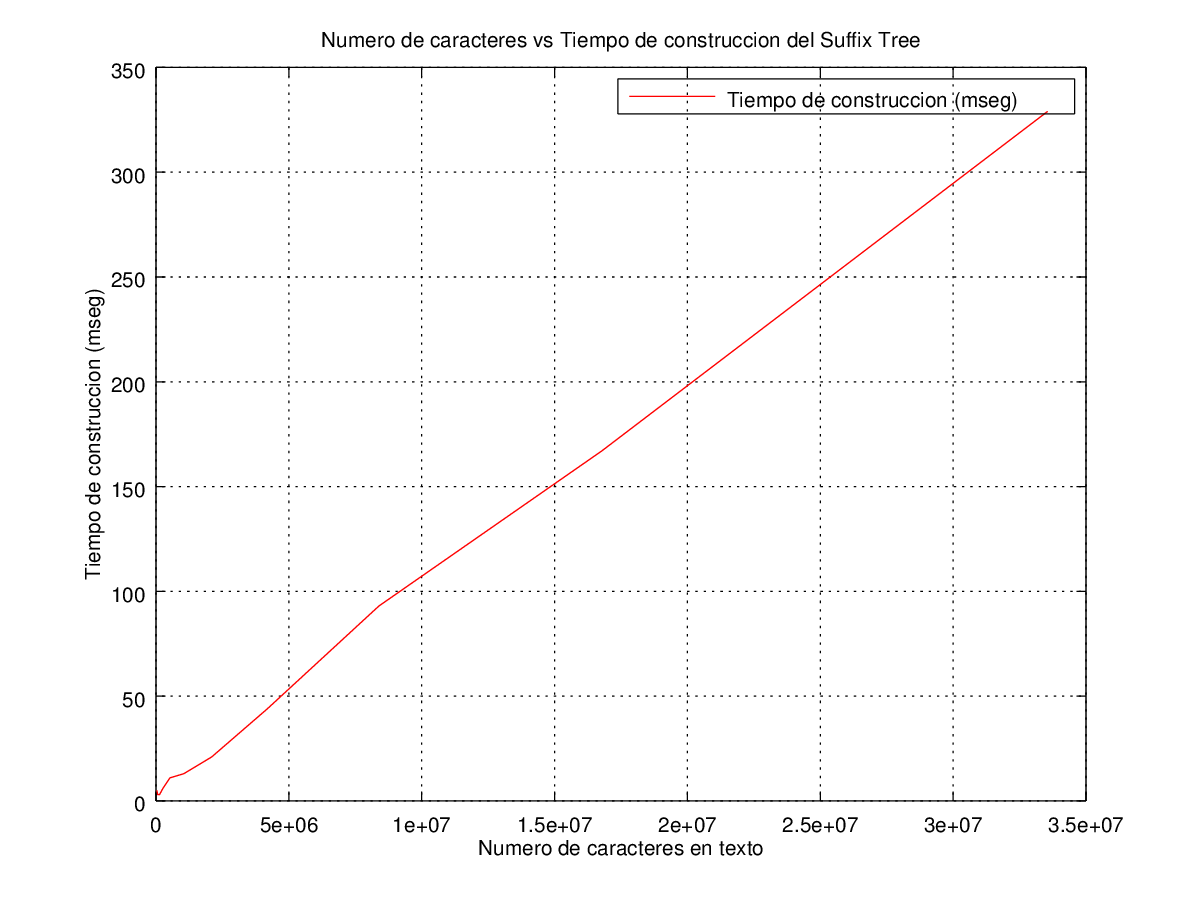
\includegraphics[width=0.8\textwidth]{fig1.png}

		Figura 1: Tiempo de creación del Suffix Tree para N = $2^{15..25}$
	\end{center}

	% % % % % % % % % % % % % % % % % % % % % % % % % % % % % % % % % % % % % % % % % % % % % % % % % % % % % % % % % % % % % % % % % % % % % % % % % % % % % % % % % % % % % % % % % %
	\newpage
	% % % % % % % % % % % % % % % % % % % % % % % % % % % % % % % % % % % % % % % % % % % % % % % % % % % % % % % % % % % % % % % % % % % % % % % % % % % % % % % % % % % % % % % % % %

	\subsection{Desempeño de operación \textit{Buscar}}

	Los resultados para los tiempos de búsqueda en el Suffix Tree son los siguientes:

	\begin{center}
		\begin{tabular}{|c|c|c|}
			\hline
			Número de palabras & Largo promedio del patrón & Tiempo de búsqueda (nano-segundos)\\
			\hline
			$2^{15}$ & 5.36 & 2671.75\\
			\hline
			$2^{16}$ & 5.31 & 1109.40\\
			\hline
			$2^{17}$ & 5.52 & 259.94\\
			\hline
			$2^{18}$ & 5.39 & 296.97\\
			\hline
			$2^{19}$ & 5.35 & 254.40\\
			\hline
			$2^{20}$ & 4.76 & 268.31\\
			\hline
			$2^{21}$ & 4.50 & 246.81\\
			\hline
			$2^{22}$ & 4.43 & 245.39\\
			\hline
			$2^{23}$ & 4.37 & 254.88\\
			\hline
			$2^{24}$ & 4.42 & 253.84\\
			\hline
			$2^{25}$ & 4.47 & 261.40\\
			\hline
		\end{tabular}
	\end{center}

	\begin{center}
		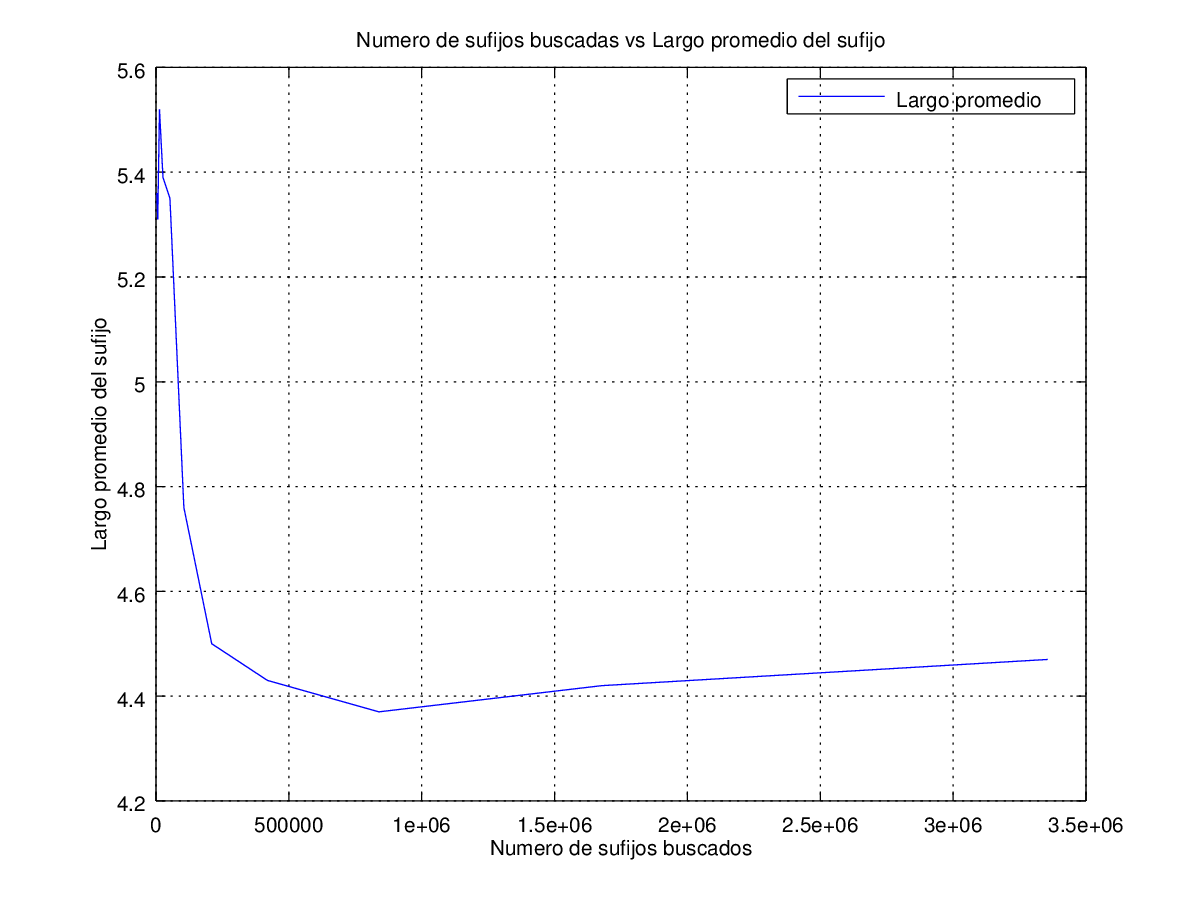
\includegraphics[width=0.8\textwidth]{fig2.png}

		Figura 2: Largo promedio del patrón
	\end{center}

	\begin{center}
		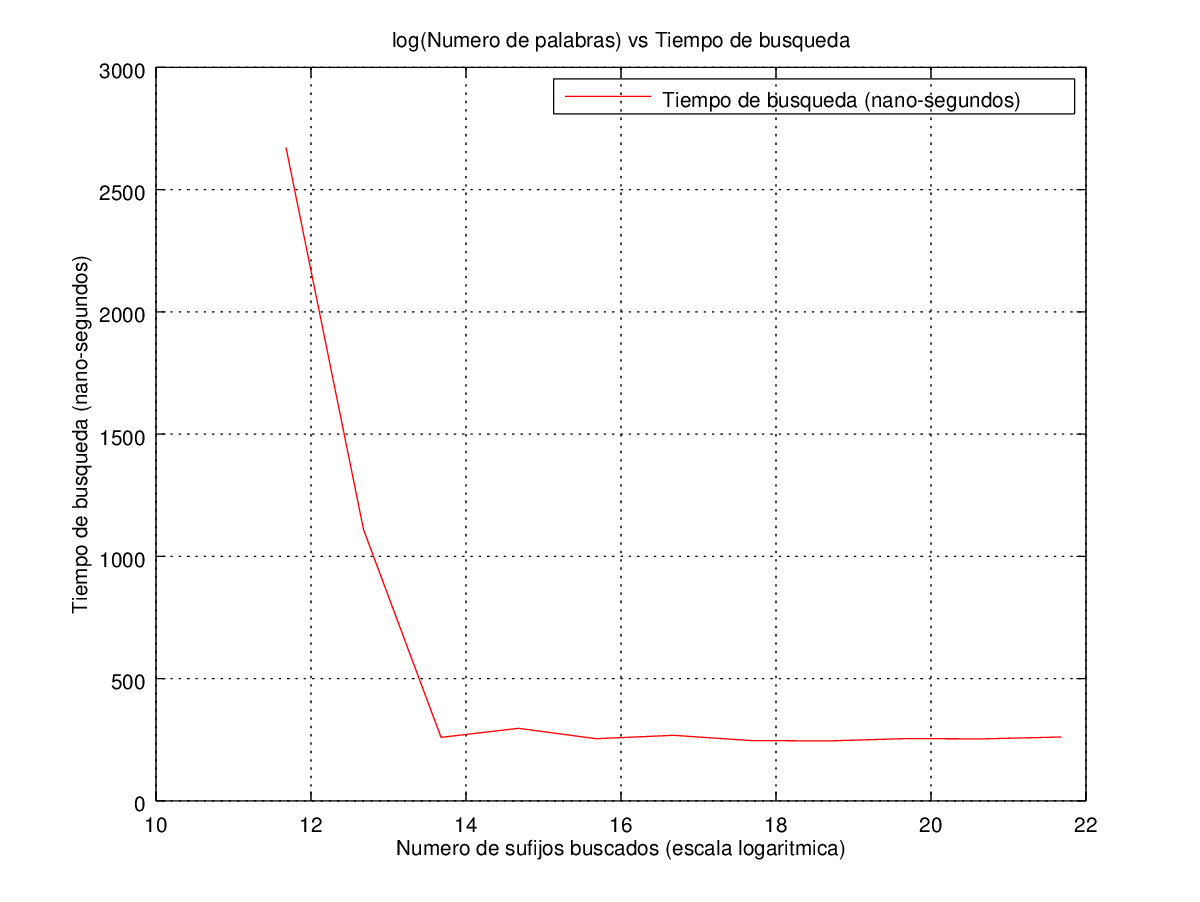
\includegraphics[width=0.8\textwidth]{fig3.png}

		Figura 3: Tiempo de búsqueda
	\end{center}

	% % % % % % % % % % % % % % % % % % % % % % % % % % % % % % % % % % % % % % % % % % % % % % % % % % % % % % % % % % % % % % % % % % % % % % % % % % % % % % % % % % % % % % % % % %
	\newpage
	% % % % % % % % % % % % % % % % % % % % % % % % % % % % % % % % % % % % % % % % % % % % % % % % % % % % % % % % % % % % % % % % % % % % % % % % % % % % % % % % % % % % % % % % % %

	\section{Análisis y Conclusiones}

	\subsection{Construcción del Suffix Tree}

	Nuestra implementación funciona bien cuando se usan palabras cortas, dado que es posible construir el Suffix Tree en tiempo $O(n)$ (puesto que al duplicar el largo de la palabra,
	también se duplicaba el tiempo en nano-segundos para construirlo).

	Nuestra hipótesis de que el \textit{garbage collector} de Java interferiría con nuestros resultados es correcta, dado que cada vez que se corría el algoritmo para una
	cantidad fija de caracteres variaba notablemente. Aún así, su interferencia es muy baja como para considerarla válida, por lo que solo lo explicamos por motivos de completitud.

	Tomando este caso, encontramos que el algoritmo de Ukkonen tarda (por ejemplo) 5 milisegundos para \\N = $2^{15}$ caracteres, y se va duplicando (aproximadamente) cada vez que duplicamos
	la cantidad de caracteres, por lo que la implementación parece haber sido conseguida en tiempo $O(n)$.

	A último momento, nos dimos cuenta que nuestra implementación tenía problemas al momento de ejecutarse con textos largos, dado que no creaba correctamente los nodos internos.
	De esta forma el arbol se creaba demasiado rápido como para ser coherente con la cantidad de enlaces que deberían existir en el Suffix Tree.

	\subsection{Búsqueda en el Suffix Tree}

	Encontramos que la búsqueda en el Suffix Tree (respecto a nuestra implementación) cae notablemente, lo que probablemente se debe a que mientras más sufijos se tienen, más sufijos se
	descartan al momento de buscar la respuesta final. Notar que en nuestra implementación, un \textbf{break} en el código \textit{bypassea} el \textit{loop}, cuando en el \textit{loop}
	se debería salir solo cuando no quedan más sufijos por procesar.

	En resumen, mientras más sufijos hay, más quedan sin procesar al momento de buscar, por lo que la cantidad de pasadas es menor.

	\subsection{Conclusiones}

	Creemos que el problema en la creación de nodos internos se debe a la creación errónea de los \textit{suffix links} o al seguimiento incorrecto de éstos.
	Las funciones de conteo están correctas para Suffix Trees bien construídos (i.e. de tamaño pequeño en nuestra implementación), pero pueden mejorarse debido a que se usa recursión para
	su implementación. Si hubieramos construído correctamente el Suffix Tree con los textos extensos de prueba, probablemente lanzaría un \textit{Stack Overflow}, por lo que en ese caso
	se cambiaría a una implementación iterativa.

\end{document}
